\section{Developing and Assessing a Quantitative Evaluation Metric for
Kernel Security}
\label{sec.metric}

\lois{I just noticed Justin made some extensive in this section. I will make some
suggestions, but we might want to touch base to see if these comments address
his concerns} The first step to addressing the threat articulated above is to establish
a metric by which kernel security can be
quantitatively evaluated. In this section we document the development of such
a metric. First, we look at current commonly used metrics for code complexity and why
they may be less than effective.
The next section discusses our proposed metric, which focuses on
using the kernel code paths accessed by %common
widely used applications. Finally, we
%show how our
use the metric to  %can be used to provide a fair
verify our central hypothesis, by testing for the presence of 40 severe Linux
 Kernel bugs.\lois{This intro section needs work. I'm not happy with what is
 here, though I think it is somewhat clearer than what was there before.}


% and their impact on the kernel, and to reveal which portions contained fewer bugs.

\subsection{Previous Risk Metrics for Software}

A contributing factor to the kernel security problem is that system
designers
still lack a standard method for quantifying the safety (or risk) of
privileged code.   \cappos{Is this really true?  No one has ever proposed
a metric?  We do need to do a more detailed analysis of this.  I would vote
to remove this sentence regardless...} \lois{ I would agree its probably best just
to get rid of the sentence. But I believe the goal here was to say that there is
no widely accepted and used standard method.}


%Structurally,
%As shown in Figure \ref{diagram/fig3.png},
The Linux kernel is divided into several main sub-systems such as %sub-directories:
%\texttt{kernel} (main kernel), \texttt{ipc} (inter-process communication),
%\texttt{net} (networking), \texttt{fs} (file system), and \texttt{device drivers} (device drivers).
process management, file system, networking, memory management and device drivers.
Chou %showed in~
\cite{PittSFIeld} demonstrated that certain functions' directories, e.g.,
\texttt{device drivers}, result in some parts of the Linux kernel having
error rates much higher than others. Kernel source code size
and age also affect how frequently errors occur in the kernel.
%largest/newest quartile of functions in kernel have error rates
%several orders of magnitude higher than the smallest/oldest quartile.
Years later, Palix found that \texttt{drivers} still contains the most faults in
the Linux kernel, in addition to HAL and \texttt{fs}~\cite{palix2011faults}.
%On the other hand,
In ~\cite{engler2001bugs} Engler analyzed system code by inferring programmer
beliefs. \lois{what does the previous sentence mean}This is achieved by static analysis
of source code that looks for contradictions, such as acquired locks are
not released. There has also been work that generates vulnerability
signatures~\cite{brumley2006towards}, which match all exploits
of a given vulnerability. Most of such work is based on a mix of static and
dynamic analysis, constraint solving and symbolic execution~\cite{chou2003static}.
However, most of these findings have not yet been used to design
secure systems.

Researchers in software engineering have also %studied and
explored different metrics to identify and predict bugs in the systems they design.
The number of lines of code has been used as one
predictor~\cite{Bug-Location}, as has a file's revision status and
whether or not the file previously contained bugs~\cite{Bug-Location,
lewis2013does}. Studies have also been conducted based on
the number of functions and/or the number of executable lines of code in
the function~\cite{Mining-Metrics}.\lois[Isn' this a bit repetitious]
Coverage-based fault localization,
on the other hand, assumes that execution events that occur mostly in failing
test cases, but rarely in passing test cases, are more \textit{suspect}
of being the fault~\cite{jones2002visualization}. Follow-up work used
the set difference of the statements covered by passing and failing test
cases with run-time events~\cite{agrawal1995fault, jones2005empirical},
and used statistical likelihood that a predicate that evaluates to True is
correlated with failure~\cite{liblit2005scalable}.

While these metrics can be useful in building models to provide a general
idea about
where bugs may be located in software systems, they have limitations.
Firstly, the metrics mentioned above are not specifically designed for
studying bugs in OS kernels.
\cappos{Why does this matter?}
Therefore, they do not take into account the way system calls are invoked
by user applications.
Moreover, these metrics can not provide information about the accurate
location of the bugs within the kernel,
which is important to our study.
\cappos{Are you going to show that this is true?  Can you explain more
about why these do not work?}
\cappos{Do existing metrics work on a LOC level?  }

Without any guidance as to what parts of the kernel are safe, past
initiatives to protect the system through isolation,
such as by building a sandbox or using library OSes, because they could not
isolate user programs effectively.  \cappos{What are you saying?}
These methods can mitigate the problem, but any such system will still
allow access to the kernel the same way as before.
They simply move the attack surface from between the user space and the
kernel, \yanyan{what's the purpose/consequence of this move? why is this
move good or bad?}
to between these new systems and the kernel, but the surface is not
necessarily reduced.
As a result, the proposed solutions do not make the systems more secure.

Recognizing this limitation, we propose a novel security metric to
quantitatively measure and evaluate the kernel for bugs and other
vulnerabilities by checking at the level of lines of code against
known kernel bugs.
With this metric, we would be better able to understand security features
of the kernel, and design an interface that is exposed to the user space
in a secure way.
Ideally,this would mean only exposing the safe portions of the kernel to
the user space.
However, in some scenarios, risky portions must be exposed to the kernel as
well.
The kernel coverage safety metric %, however,
 can provide us guidance about the potential dangers and
can help us safely-reimplement those risky kernel interface (or system
calls) to avoid the potential damage.\lois{does the metric itself tell us HOW
to safely-reimplment? Or just tell us whether it needs this reimplementation?}
%\yanyan{I don't think the new metric alerts us tho. maybe say it provides
%as a guidance which parts are risky?}

\cappos{end of text}


\subsection{Key Hypothesis}

Our hypothesis is that kernel paths executed by popular applications,
such as Web browsers or text editors, are likely to contain fewer
exploitable bugs
than uncommonly used paths. %Our reasoning is that,
Because they are frequently used, bugs and vulnerabilities in these common kernel paths
would have most likely been caught by developers.

Note that this does more than indicate which system calls are "safe."
 \gholami{I dont understand this sentence}
The proposed metric also excludes odd execution paths
through popular system calls.
This means that the chances to harbor kernel bugs in those commonly used
kernel paths are slim indeed.\lois{did proposed edit make this clearer? }

\subsection{Foundation for the Metric: Capturing and Evaluating Kernel Traces}

The first step in proving our hypothesis was to capture the lines of kernel
code executed
when running applications. The OS kernel code is organized under different
kernel directories.
Whenever an application tries to access system resources, such as file
system, I/O and memory, the kernel code under the corresponding paths is executed. Therefore,
its code execution reflects the basic behavior of the kernel, in response
to user application requests.
Our metric first identified and captured which lines of code in the kernel
were executed
when running a user program. We named the resulting captured lines of
code a \textit{kernel trace}.
A kernel trace is closely related to the program that generated the trace, so
by using the kernel traces, a comparison between different
security systems is possible.
To capture the kernel trace, we used \texttt{gcov} \cite{gcov}, a program profiling
tool that is a standard utility with the GNU compiler collection
%(GCC)
suite.


The second step was to evaluate security aspects of the captured kernel traces.% thatwe captured.
Using the historical kernel vulnerability reports, we collected a list of
severe kernel bugs from
the National Vulnerability Database, the U.S. government repository of
standards-based \yanyan{what does standards-based mean?}
\yiwen{It means there are quantitative standards provided, for example,
a vulnerability severity score.}
vulnerability management data \cite{NVD}. We analyzed the bugs as
follows. For each bug, we identified the lines of code
in the kernel that would trigger it. This can be done by examining
a patch of the Linux kernel source code to fix the bug. From the patch,
we can identify \textit{which lines of kernel code need to be modified in order to
remove the bug}.
A user program that executes the lines of code changed by a patch to fix a
kernel bug is considered to have the \textit{potential to exploit that flaw}.

We determined that the lines of code in the kernel would be risky
if they triggered one or more kernel vulnerability. Other lines of code
that did not trigger a vulnerability are considered to be safe. We empirically
 labeled the lines of code in the kernel that contain no bugs as "safe lines"
using the above kernel trace analysis.
The safe lines of code would then compose the safe portion of the kernel, which can be trusted to build a secure trusted computing base for secure systems.

\subsection{Verification of Hypothesis}
\label{Verification-of-Hypothesis}

To verify our hypothesis that commonly used kernel paths contain fewer bugs,
we identified these paths as a subset of the total reachable kernel paths as follows.

%\begin{enumerate}
First, common paths were captured by running the most widely used applications
or open-source libraries, as shown in Figure \ref{diagram/data_collection.png}.
These data collection phase experiments included running several applications,
such as two large-scale browsers (Mozilla Firefox and Google Chrome)
 over \texttt{gcov}. Experiments also included running 50 packages among
 the top 200 popular Debian packages \cite{Top-Packages}
 in a Linux kernel version 3.14.1.

%During this step, we conducted
Several other operations needed to access common paths were conducted, including
intensive file management tasks to create/read/update or delete files and
directories from the underlying filesystem. These tests were completed
during a discrete period of 20 hours over 5 days.

Next, the total reachable paths were captured by comprehensive system call
fuzzing and by running the Linux kernel test suite. These experiments helped
 to capture the total reachable paths in the kernel as thoroughly as possible.

Two approaches were used to capture this trace.

\begin{itemize}
\item System call fuzzing experiments were designed to utilize the Trinity
 system call fuzz tester \cite{Trinity}. These included sequential execution of more than 300 system calls with 1 million iterations for executing each system call by 16 child processes as Trinity workers. The obtained kernel trace comprehensively reflected various aspects of the kernel functionalities.

%File management and network system calls, \yanyan{what is file management?} which gave us a thorough kernel trace.

\item Linux Test Project (LTP) \cite{LTP} was used to capture the total reachable kernel trace.
Linux Test Project is a mature and well maintained tool to test the Linux
kernel.
We ran all the available system call test cases with this tool to capture
the kernel trace.

We used LTP in addition to Trinity in order to validate the kernel trace generated
by Trinity, as well as to catch the traces it might miss.
In our experiments, the LTP was able to capture about 20\% of kernel trace
that were missed by Trinity, while Trinity provided us about 15\% of kernel trace
that were not included by LTP.
\end{itemize}

Figure \ref{fig:datacollection} shows different platforms and tools that were used
 for the analysis. The kernel traces are generated by running several legacy
  applications, system fuzzers and LTP within different platforms such as
  Lind (Nacl/Repy), virtualized platforms and a normal native Linux. Then a Python
   analyzer program filters and transforms the kernel traces that are collected
    using gcov. The output will be used for kernel traces analysis as
    discussed in the following sections.

\begin{figure}%[h]
\centering
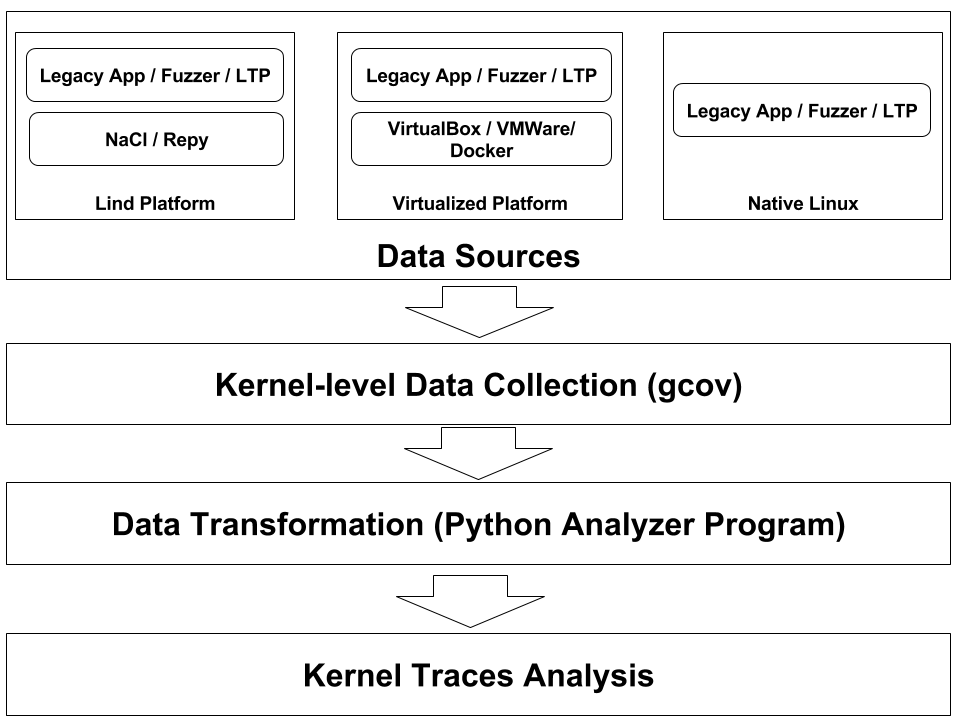
\includegraphics[width=1.0\columnwidth]{diagram/data_collection.png}
\caption{Various activities that were performed to capture and analyze the kernel
 traces generated by legacy applications, system fuzzers, LTP, and CVE bug
 reports. The traces are collected using \texttt{gcov} and a Python-based
 program that will be transformed lois{transformed to what? And, how?}
 for final data analysis.}
\label{fig:datacollection}
\end{figure}



We were able to assess
%access our
the total reachable kernel paths through combining the kernel traces generated by Trinity and LTP. The results show that 38.5\% of the total reachable
kernel paths are commonly used.
More importantly, only 2.5\% of the bugs examined were found in the common
paths,
while 50\% of the bugs were found in the total reachable kernel paths.
%Our
The results strongly suggest that common paths may contain fewer bugs than uncommon
paths. \yanyan{I feel this is a bit early to make this conclusion.}
\lois{does the slight wording change answer your concern, Yanyan?}

\subsubsection{Coverage Analysis of Common Paths}

The kernel trace coverage of the common paths and the total reachable paths
are shown in Table \ref{table:kernel_coverage}.|lois{Isn't this FIGURE 2, not
Table 2}
The results show that the size of commonly-used kernel paths is small,
merely 12.4\% of the entire kernel code base.
The common paths coverage is also significantly smaller than the total
reachable paths coverage
(about 1/3 of the entire kernel).

It may appear surprising that the total reachable paths coverage is low,
and accounts for only about one-third of the entire kernel.  However,
this is consistent with kernel code coverage analysis
measurements conducted by other researchers \cite{LTP-Coverage}.
One reason that this occurs is that many paths
in the kernel cannot be accessed from the system call API. Another reason
is that
while obtaining the kernel coverage data, as most researchers did, we used
a system call fuzzing tool
and a Linux test suite to generate the kernel trace. These existing
tools do not reach every possible path in the kernel, due to
the fact that there are some limitations on the iteration number of issuing
the fuzzing calls. In addition, some kernel paths can only be reached by
certain combinations of different function calls with specific arguments.


\begin{figure}%[h]
\centering
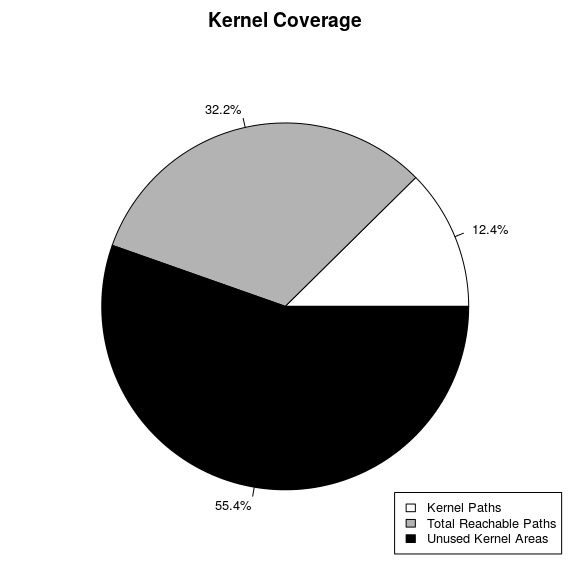
\includegraphics[width=1.0\columnwidth]{diagram/kernelcoverage.png}
\caption{Percentage of different kernel areas that were reached during
 LTP and Trinity experiments.}
\label{fig:coverage}
\end{figure}


%Although the total reachable paths coverage is not 100\% of the entire
%kernel code base,
%it is still very large and contains many bugs.
%However, because the commonly used kernel path coverage is much smaller
%than
%the total reachable path coverage, this is a positive indication that these
%relatively small areas can be considered safe.

%\begin{table}
%\centering
%\scriptsize
%\caption {Kernel Coverage}
%\begin{tabular}{|l|c|}
%  \hline
%  \textbf{Kernel Paths} & \textbf{Kernel Coverage (percentage)} \\
%  \hline \hline
%  Common Paths & 12.4\% \\
%  \hline
%  Total Reachable Paths & 32.2\% \\
%  \hline
%\end{tabular}
%\label{table:kernel_coverage}
%\end{table}

The results from Figure \ref{fig:subset} and Figure
\ref{fig:key_paths_trace}
show that the common paths are a subset of the
total reachable paths.
In Figure \ref{fig:subset} and Figure \ref{fig:key_paths_trace},
the ``OverlappedLines'' indicate the lines of code
in the kernel that appear both in the common paths and the total reachable
paths. While the ``UniqueLines'' show the lines of code that only appear in
the total reachable paths.

In Figure \ref{fig:subset}, the ``UniqueLines''
represent a large portion of the total reachable paths, more than 90K LOC.
Those lines of code are not executed by popular applications, which can be
potentially dangerous.

In Figure \ref{fig:key_paths_trace}, \texttt{fs}, \texttt{kernel/sched},
and \texttt{mm} refer to the total number of lines of code in that Linux kernel path.
Figure \ref{fig:key_paths_trace} shows that
substantial amount of code are found only inside the total reachable paths,
for some essential kernel paths like \texttt{fs} (6.5K LOC),
\texttt{kernel/sched} (3K LOC),
and \texttt{mm} (8K LOC).
A main reason for this outcome is that many lines of code in those kernel paths
are inside if conditions, and can only be reached by using special or
rare arguments and flags. Since the daily-used operations of
the popular applications do not require those kind of rare arguments
and flags, those ``UniqueLines'' only exist in the total reachable paths.

We closely examined the kernel trace derived from common paths
and the total reachable paths. We found that for each different path
in the kernel, the lines of code
in the common paths trace also appeared in the total reachable paths trace.
But there are many lines of code (more than 50\%)
in the total reachable paths trace that are not in the common paths. This
shows that the common paths trace and
the total reachable paths we obtained are as expected, because common paths in
the kernel should definitely be reachable. \yanyan{how to define correct?}
\lois{again, Yanyan, does the word change from "correct" to "as expected" help?}
One further finding is that the common paths account
for only 38.5\% of the total reachable paths.
This suggests that a large portion (61.5\%) of the kernel is not frequently
used by popular applications on a daily basis.

\begin{figure}
\centering
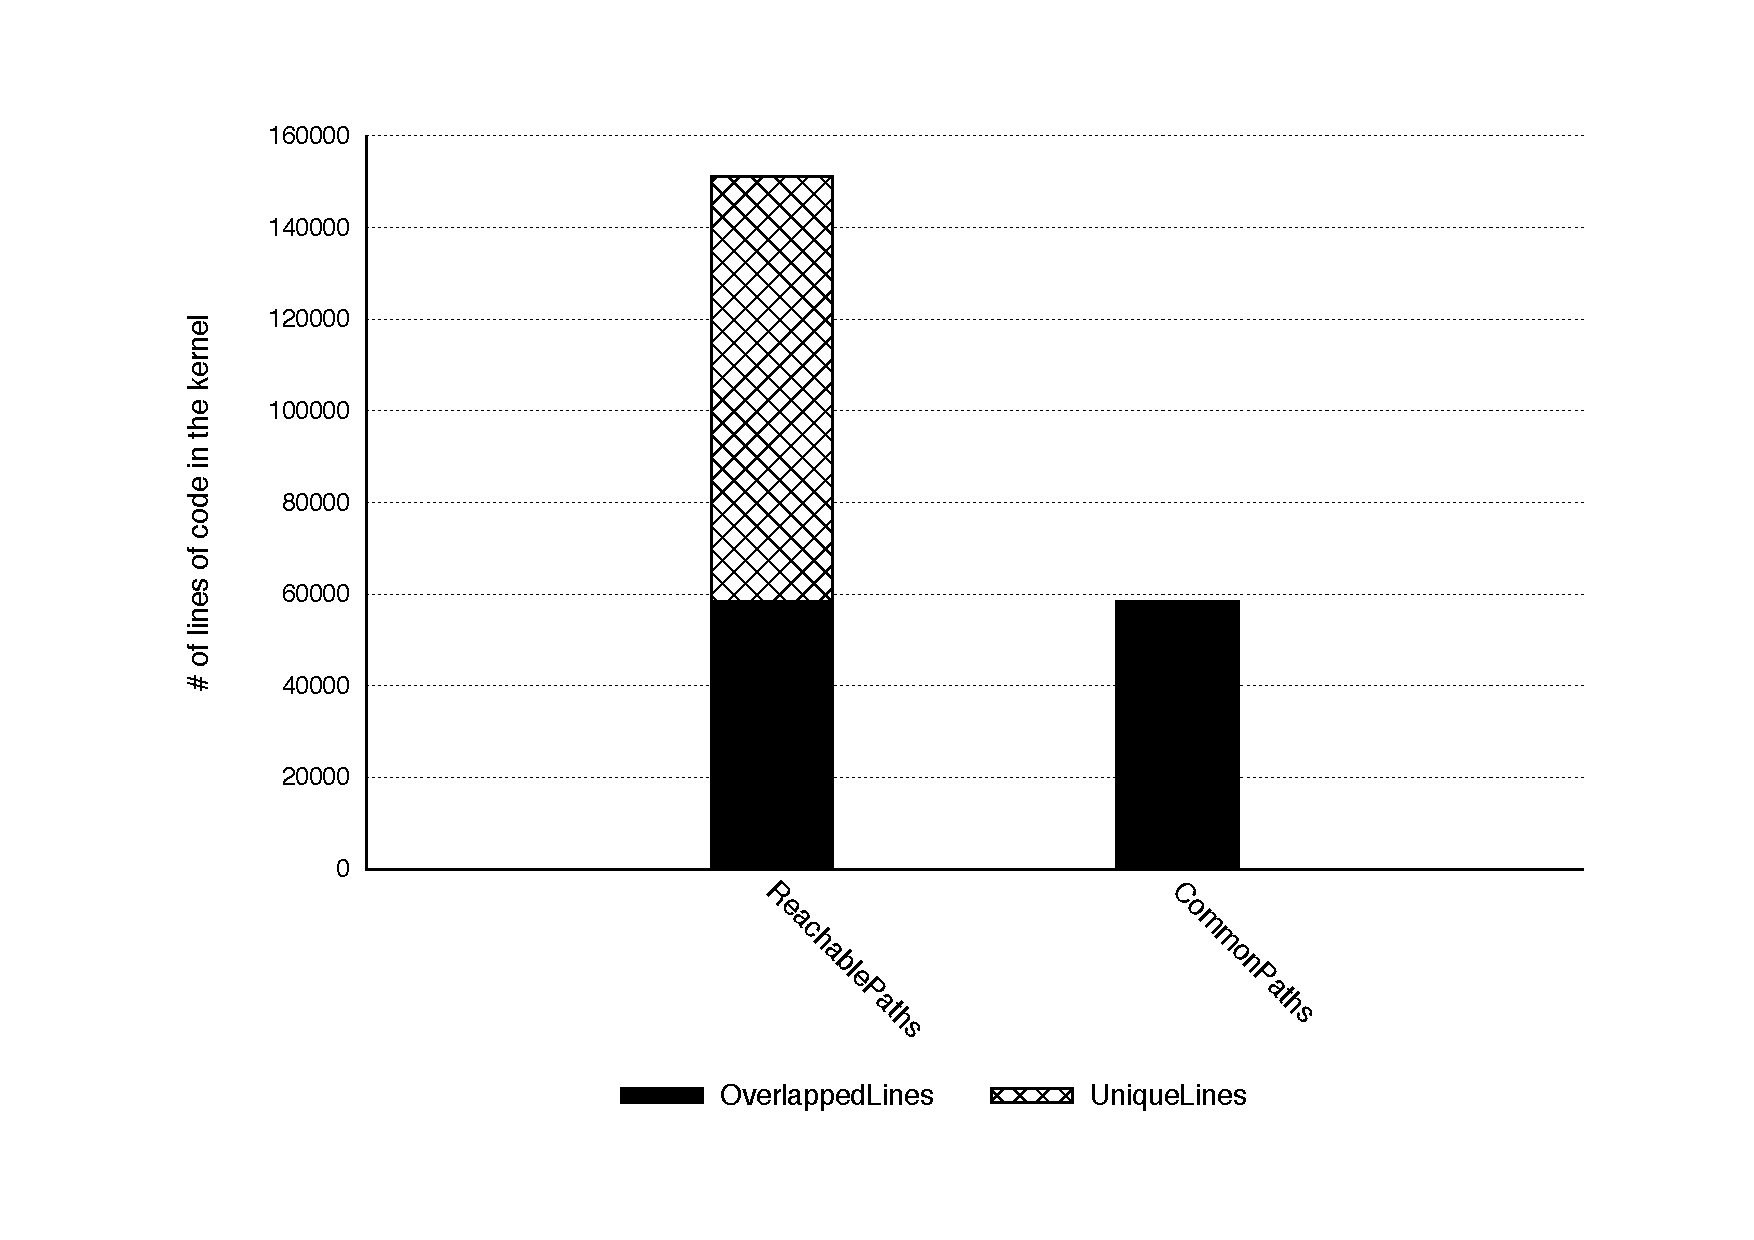
\includegraphics[width=1.0\columnwidth]{diagram/lind_oakland16_diagram_01.pdf}
\caption{Kernel Trace Comparison: Common paths as a subset of reachable
paths}
\label{fig:subset}
\end{figure}

\begin{figure}
\centering
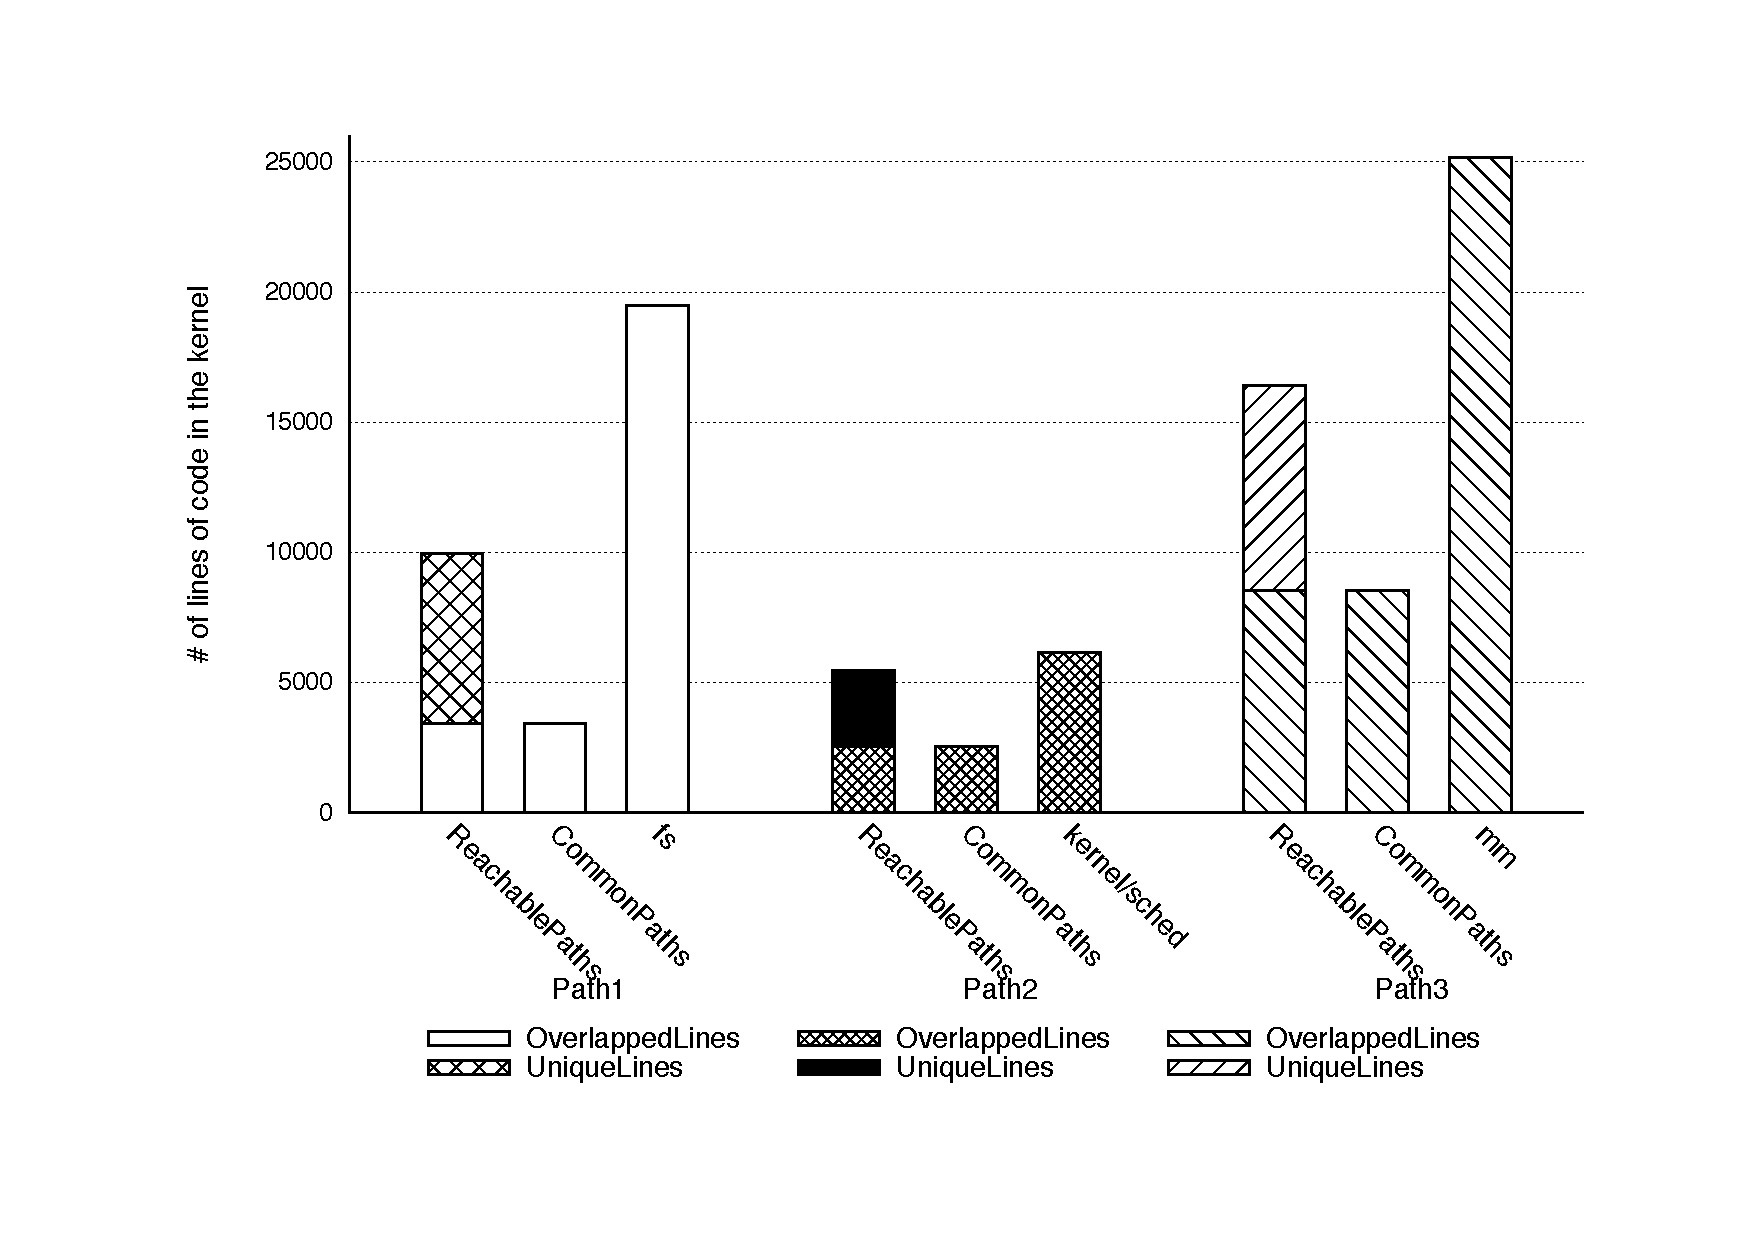
\includegraphics[width=1.0\columnwidth]{diagram/lind_oakland16_diagram_02.pdf}
\caption{Kernel Trace in Key Paths}
\label{fig:key_paths_trace}
\end{figure}

\subsubsection{Security Analysis of Kernel Paths\textendash Locating the
Risky Portions}

To verify our hypothesis, we next checked which portions of
the kernel contained kernel bugs. We examined 40 severe Linux kernel
bugs that had been discovered by the research community in the last five
years (the first two columns in Table
\ref{table:vulnerabilities_commonly_used_kernel_paths}).
Those 40 bugs were chosen from the NVD bug database, according to
the vulnerability severity score assigned to them. We started with the ones
that have the highest severity score.
We used these kernel bugs to check if vulnerabilities existed in certain
kernel traces. This is done by comparing the kernel traces with the lines
of code we labeled for each bug, based on change of lines in the
kernel patch.
The results of our experiment are shown the last two columns in Table
\ref{table:vulnerabilities_commonly_used_kernel_paths}.

\begin{table*}[!ht]
\scriptsize
\centering

\caption {Linux Kernel Bugs, and Vulnerabilities in Different Portions of
the Kernel
({\color{red}\ding{51}}: vulnerability in paths; \ding{55}: vulnerability
not in paths)}

\begin{tabular}{|l|l|c|c|}\hline
\multirow{2}{*}{\textbf{Vulnerability}} & \multirow{2}{*}{\textbf{Specific
Type}} & \multicolumn{2}{c|}{\bf Portion of the Kernel} \\
\cline{3-4}
&  & \textbf{Total Reachable Paths} &  \textbf{Common Paths} \\ \hline

 CVE-2014-9529 & concurrency, race condition & {\color{red}\ding{51}} &
\ding{55} \\
 CVE-2014-3631 & NULL pointer dereference & {\color{red}\ding{51}} &
\ding{55} \\
 CVE-2012-6657 & network socket variable mischeck & {\color{red}\ding{51}}
& \ding{55} \\
 CVE-2014-5207 & privilege escalation & \ding{55} & \ding{55} \\
 CVE-2014-5206 & privilege escalation & \ding{55} & \ding{55} \\
 CVE-2014-3153 & privilege escalation & \ding{55} & \ding{55} \\
 CVE-2014-2851 & privilege escalation & \ding{55} & \ding{55} \\
 CVE-2014-2706 & race condition, DoS & {\color{red}\ding{51}} & \ding{55}
\\
 CVE-2014-0100 & race condition, DoS & {\color{red}\ding{51}} & \ding{55}
\\
 CVE-2014-0049 & buffer overflow & \ding{55} & \ding{55} \\
 CVE-2012-6638 & DoS & {\color{red}\ding{51}} & \ding{55} \\
 CVE-2014-0038 & privilege escalation & \ding{55} & \ding{55} \\
 CVE-2013-6368 & privilege escalation & \ding{55} & \ding{55} \\
 CVE-2013-4587 & index error, privilege escalation & \ding{55} & \ding{55}
\\
 CVE-2013-4563 & size/boundary check, DoS & {\color{red}\ding{51}} &
\ding{55} \\
 CVE-2013-4348 & value validation error & \ding{55} & \ding{55} \\
 CVE-2013-4300 & privilege escalation & {\color{red}\ding{51}} & \ding{55}
\\
 CVE-2013-1943 & privilege escalation & \ding{55} & \ding{55} \\
 CVE-2013-2094 & privilege escalation & {\color{red}\ding{51}} & \ding{55}
\\
 CVE-2013-3301 & NULL pointer dereference, DoS & {\color{red}\ding{51}} &
\ding{55} \\
 CVE-2013-1858 & privilege escalation & {\color{red}\ding{51}} & \ding{55}
\\
 CVE-2013-1797 & use-after-free & {\color{red}\ding{51}} & \ding{55} \\
 CVE-2013-1763 & privilege escalation, index error & \ding{55} & \ding{55}
\\
 CVE-2013-0310 & NULL pointer dereference & \ding{55} & \ding{55} \\
 CVE-2012-2136 & heap-based buffer overflow & \ding{55} & \ding{55} \\
 CVE-2012-2100 & lack of sanity check  & \ding{55} & \ding{55} \\
 CVE-2012-0028 & privilege escalation & {\color{red}\ding{51}} & \ding{55}
\\
 CVE-2011-2517 & privilege escalation, buffer overflow &
{\color{red}\ding{51}} & \ding{55} \\
 CVE-2012-2123 & privilege escalation  & {\color{red}\ding{51}} & \ding{55}
\\
 CVE-2012-1146 & NULL pointer dereference  & \ding{55} & \ding{55} \\
 CVE-2012-0207 & divide-by-zero error and panic & \ding{55} & \ding{55} \\
 CVE-2011-2525 & NULL pointer dereference  & {\color{red}\ding{51}} &
\ding{55} \\
 CVE-2011-1076 & NULL pointer dereference  & {\color{red}\ding{51}} &
\ding{55} \\
 CVE-2011-2184 & NULL pointer dereference, none initialization & \ding{55}
& \ding{55} \\
 CVE-2010-2478 & integer overflow & {\color{red}\ding{51}} & \ding{55} \\
 CVE-2010-2960 & NULL pointer dereference  & \ding{55} & \ding{55} \\
 CVE-2010-2492 & privilege escalation, buffer overflow & \ding{55} &
\ding{55} \\
 CVE-2010-2240 & stack overflow & {\color{red}\ding{51}} &
{\color{red}\ding{51}}\\
 CVE-2010-1188 & use-after-free & \ding{55} & \ding{55} \\
 CVE-2010-0437 & NULL pointer dereference  & {\color{red}\ding{51}} &
\ding{55} \\ \hline
 \multicolumn{2}{|c|}{\bf Percentage contains bugs} & {\bf $50\%$} & {\bf
$2.5\%$} \\ \hline
\end{tabular}
\label{table:vulnerabilities_commonly_used_kernel_paths}
\end{table*}

The results of this analysis suggest that commonly used kernel paths contain only
2.5\% of the bugs we had targeted.
Since the total reachable kernel paths contain 50\% of the bugs that were
examined in this paper,
it can be inferred that commonly used kernel paths clearly contain fewer bugs
than other portions of the kernel.

We chose our bugs from the large-scale NVD database, which includes representative
bugs for all categories. In choosing the bugs, we
started with ones assigned the highest vulnerability severity scores.
Therefore, we believe that our sample was not biased, and should be representative
to reflect the general distribution of bugs in the Linux kernel. \lois{Why does this
method, which seems less than random, prove it is not biased?}

Our hypothesis and findings provide insights and guidelines for new designs
of secure systems,
which will be discussed in the next section.
\cappos{Is this statistically significant?}
\yiwen{I added something to explain our bug sample dataset.
More knowledge of statistics may be required. I will think about it more.}
